% Options for packages loaded elsewhere
% Options for packages loaded elsewhere
\PassOptionsToPackage{unicode}{hyperref}
\PassOptionsToPackage{hyphens}{url}
\PassOptionsToPackage{dvipsnames,svgnames,x11names}{xcolor}
%
\documentclass[
  spanish,
  11pt,
  a4paper,
  DIV=11,
  numbers=noendperiod]{scrartcl}
\usepackage{xcolor}
\usepackage[margin=2.5cm]{geometry}
\usepackage{amsmath,amssymb}
\setcounter{secnumdepth}{5}
\usepackage{iftex}
\ifPDFTeX
  \usepackage[T1]{fontenc}
  \usepackage[utf8]{inputenc}
  \usepackage{textcomp} % provide euro and other symbols
\else % if luatex or xetex
  \usepackage{unicode-math} % this also loads fontspec
  \defaultfontfeatures{Scale=MatchLowercase}
  \defaultfontfeatures[\rmfamily]{Ligatures=TeX,Scale=1}
\fi
\usepackage{lmodern}
\ifPDFTeX\else
  % xetex/luatex font selection
  \setmainfont[]{Times New Roman}
\fi
% Use upquote if available, for straight quotes in verbatim environments
\IfFileExists{upquote.sty}{\usepackage{upquote}}{}
\IfFileExists{microtype.sty}{% use microtype if available
  \usepackage[]{microtype}
  \UseMicrotypeSet[protrusion]{basicmath} % disable protrusion for tt fonts
}{}
\makeatletter
\@ifundefined{KOMAClassName}{% if non-KOMA class
  \IfFileExists{parskip.sty}{%
    \usepackage{parskip}
  }{% else
    \setlength{\parindent}{0pt}
    \setlength{\parskip}{6pt plus 2pt minus 1pt}}
}{% if KOMA class
  \KOMAoptions{parskip=half}}
\makeatother
% Make \paragraph and \subparagraph free-standing
\makeatletter
\ifx\paragraph\undefined\else
  \let\oldparagraph\paragraph
  \renewcommand{\paragraph}{
    \@ifstar
      \xxxParagraphStar
      \xxxParagraphNoStar
  }
  \newcommand{\xxxParagraphStar}[1]{\oldparagraph*{#1}\mbox{}}
  \newcommand{\xxxParagraphNoStar}[1]{\oldparagraph{#1}\mbox{}}
\fi
\ifx\subparagraph\undefined\else
  \let\oldsubparagraph\subparagraph
  \renewcommand{\subparagraph}{
    \@ifstar
      \xxxSubParagraphStar
      \xxxSubParagraphNoStar
  }
  \newcommand{\xxxSubParagraphStar}[1]{\oldsubparagraph*{#1}\mbox{}}
  \newcommand{\xxxSubParagraphNoStar}[1]{\oldsubparagraph{#1}\mbox{}}
\fi
\makeatother

\usepackage{color}
\usepackage{fancyvrb}
\newcommand{\VerbBar}{|}
\newcommand{\VERB}{\Verb[commandchars=\\\{\}]}
\DefineVerbatimEnvironment{Highlighting}{Verbatim}{commandchars=\\\{\}}
% Add ',fontsize=\small' for more characters per line
\usepackage{framed}
\definecolor{shadecolor}{RGB}{241,243,245}
\newenvironment{Shaded}{\begin{snugshade}}{\end{snugshade}}
\newcommand{\AlertTok}[1]{\textcolor[rgb]{0.68,0.00,0.00}{#1}}
\newcommand{\AnnotationTok}[1]{\textcolor[rgb]{0.37,0.37,0.37}{#1}}
\newcommand{\AttributeTok}[1]{\textcolor[rgb]{0.40,0.45,0.13}{#1}}
\newcommand{\BaseNTok}[1]{\textcolor[rgb]{0.68,0.00,0.00}{#1}}
\newcommand{\BuiltInTok}[1]{\textcolor[rgb]{0.00,0.23,0.31}{#1}}
\newcommand{\CharTok}[1]{\textcolor[rgb]{0.13,0.47,0.30}{#1}}
\newcommand{\CommentTok}[1]{\textcolor[rgb]{0.37,0.37,0.37}{#1}}
\newcommand{\CommentVarTok}[1]{\textcolor[rgb]{0.37,0.37,0.37}{\textit{#1}}}
\newcommand{\ConstantTok}[1]{\textcolor[rgb]{0.56,0.35,0.01}{#1}}
\newcommand{\ControlFlowTok}[1]{\textcolor[rgb]{0.00,0.23,0.31}{\textbf{#1}}}
\newcommand{\DataTypeTok}[1]{\textcolor[rgb]{0.68,0.00,0.00}{#1}}
\newcommand{\DecValTok}[1]{\textcolor[rgb]{0.68,0.00,0.00}{#1}}
\newcommand{\DocumentationTok}[1]{\textcolor[rgb]{0.37,0.37,0.37}{\textit{#1}}}
\newcommand{\ErrorTok}[1]{\textcolor[rgb]{0.68,0.00,0.00}{#1}}
\newcommand{\ExtensionTok}[1]{\textcolor[rgb]{0.00,0.23,0.31}{#1}}
\newcommand{\FloatTok}[1]{\textcolor[rgb]{0.68,0.00,0.00}{#1}}
\newcommand{\FunctionTok}[1]{\textcolor[rgb]{0.28,0.35,0.67}{#1}}
\newcommand{\ImportTok}[1]{\textcolor[rgb]{0.00,0.46,0.62}{#1}}
\newcommand{\InformationTok}[1]{\textcolor[rgb]{0.37,0.37,0.37}{#1}}
\newcommand{\KeywordTok}[1]{\textcolor[rgb]{0.00,0.23,0.31}{\textbf{#1}}}
\newcommand{\NormalTok}[1]{\textcolor[rgb]{0.00,0.23,0.31}{#1}}
\newcommand{\OperatorTok}[1]{\textcolor[rgb]{0.37,0.37,0.37}{#1}}
\newcommand{\OtherTok}[1]{\textcolor[rgb]{0.00,0.23,0.31}{#1}}
\newcommand{\PreprocessorTok}[1]{\textcolor[rgb]{0.68,0.00,0.00}{#1}}
\newcommand{\RegionMarkerTok}[1]{\textcolor[rgb]{0.00,0.23,0.31}{#1}}
\newcommand{\SpecialCharTok}[1]{\textcolor[rgb]{0.37,0.37,0.37}{#1}}
\newcommand{\SpecialStringTok}[1]{\textcolor[rgb]{0.13,0.47,0.30}{#1}}
\newcommand{\StringTok}[1]{\textcolor[rgb]{0.13,0.47,0.30}{#1}}
\newcommand{\VariableTok}[1]{\textcolor[rgb]{0.07,0.07,0.07}{#1}}
\newcommand{\VerbatimStringTok}[1]{\textcolor[rgb]{0.13,0.47,0.30}{#1}}
\newcommand{\WarningTok}[1]{\textcolor[rgb]{0.37,0.37,0.37}{\textit{#1}}}

\usepackage{longtable,booktabs,array}
\usepackage{calc} % for calculating minipage widths
% Correct order of tables after \paragraph or \subparagraph
\usepackage{etoolbox}
\makeatletter
\patchcmd\longtable{\par}{\if@noskipsec\mbox{}\fi\par}{}{}
\makeatother
% Allow footnotes in longtable head/foot
\IfFileExists{footnotehyper.sty}{\usepackage{footnotehyper}}{\usepackage{footnote}}
\makesavenoteenv{longtable}
\usepackage{graphicx}
\makeatletter
\newsavebox\pandoc@box
\newcommand*\pandocbounded[1]{% scales image to fit in text height/width
  \sbox\pandoc@box{#1}%
  \Gscale@div\@tempa{\textheight}{\dimexpr\ht\pandoc@box+\dp\pandoc@box\relax}%
  \Gscale@div\@tempb{\linewidth}{\wd\pandoc@box}%
  \ifdim\@tempb\p@<\@tempa\p@\let\@tempa\@tempb\fi% select the smaller of both
  \ifdim\@tempa\p@<\p@\scalebox{\@tempa}{\usebox\pandoc@box}%
  \else\usebox{\pandoc@box}%
  \fi%
}
% Set default figure placement to htbp
\def\fps@figure{htbp}
\makeatother



\ifLuaTeX
\usepackage[bidi=basic]{babel}
\else
\usepackage[bidi=default]{babel}
\fi
\ifPDFTeX
\else
\babelfont{rm}[]{Times New Roman}
\fi
% get rid of language-specific shorthands (see #6817):
\let\LanguageShortHands\languageshorthands
\def\languageshorthands#1{}


\setlength{\emergencystretch}{3em} % prevent overfull lines

\providecommand{\tightlist}{%
  \setlength{\itemsep}{0pt}\setlength{\parskip}{0pt}}



 


\usepackage[hidelinks]{hyperref}
\KOMAoption{captions}{tableheading}
\makeatletter
\@ifpackageloaded{caption}{}{\usepackage{caption}}
\AtBeginDocument{%
\ifdefined\contentsname
  \renewcommand*\contentsname{Tabla de contenidos}
\else
  \newcommand\contentsname{Tabla de contenidos}
\fi
\ifdefined\listfigurename
  \renewcommand*\listfigurename{Listado de Figuras}
\else
  \newcommand\listfigurename{Listado de Figuras}
\fi
\ifdefined\listtablename
  \renewcommand*\listtablename{Listado de Tablas}
\else
  \newcommand\listtablename{Listado de Tablas}
\fi
\ifdefined\figurename
  \renewcommand*\figurename{Figura}
\else
  \newcommand\figurename{Figura}
\fi
\ifdefined\tablename
  \renewcommand*\tablename{Tabla}
\else
  \newcommand\tablename{Tabla}
\fi
}
\@ifpackageloaded{float}{}{\usepackage{float}}
\floatstyle{ruled}
\@ifundefined{c@chapter}{\newfloat{codelisting}{h}{lop}}{\newfloat{codelisting}{h}{lop}[chapter]}
\floatname{codelisting}{Listado}
\newcommand*\listoflistings{\listof{codelisting}{Listado de Listados}}
\makeatother
\makeatletter
\makeatother
\makeatletter
\@ifpackageloaded{caption}{}{\usepackage{caption}}
\@ifpackageloaded{subcaption}{}{\usepackage{subcaption}}
\makeatother
\usepackage{bookmark}
\IfFileExists{xurl.sty}{\usepackage{xurl}}{} % add URL line breaks if available
\urlstyle{same}
\hypersetup{
  pdftitle={PCA-NMDS},
  pdfauthor={Santos G},
  pdflang={es},
  colorlinks=true,
  linkcolor={blue},
  filecolor={Maroon},
  citecolor={Blue},
  urlcolor={Blue},
  pdfcreator={LaTeX via pandoc}}


\title{PCA-NMDS}
\author{Santos G}
\date{}
\begin{document}
\maketitle

\renewcommand*\contentsname{Tabla de contenidos}
{
\hypersetup{linkcolor=}
\setcounter{tocdepth}{2}
\tableofcontents
}

\section{Contexto de proyecto
(PCA-NMDS)}\label{contexto-de-proyecto-pca-nmds}

El objetivo de este bloque es aplicar un Análisis de Componentes
Principales (PCA) a variables morfométricas para resumir la variación
multivariada en pocos ejes interpretables. El PCA ayudará a reducir la
dimensionalidad, identificar correlaciones entre rasgos y construir
índices compuestos que puedan usarse en modelos posteriores o informes
técnicos.

El NMDS se aplicará sobre una matriz de abundancia de especies, con el
propósito de evaluar la similitud entre sitios de muestreo y explorar
posibles gradientes ecológicos subyacentes, complementando el enfoque
morfométrico del PCA con una perspectiva basada en la composición
comunitaria.

\section{Carga de librerías y
dataset}\label{carga-de-libreruxedas-y-dataset}

\begin{Shaded}
\begin{Highlighting}[numbers=left,,]
\CommentTok{\# Librerías}
\FunctionTok{library}\NormalTok{(tidyverse)}
\FunctionTok{library}\NormalTok{(janitor)}
\FunctionTok{library}\NormalTok{(knitr)}
\FunctionTok{library}\NormalTok{(vegan)}
\FunctionTok{library}\NormalTok{(ggrepel) }
\FunctionTok{library}\NormalTok{(MVN)}
\FunctionTok{library}\NormalTok{(psych)}
\FunctionTok{library}\NormalTok{(ggcorrplot)}
\FunctionTok{library}\NormalTok{(palmerpenguins) }

\CommentTok{\# Cargar dataset}
\NormalTok{df\_raw }\OtherTok{\textless{}{-}}\NormalTok{ penguins }\SpecialCharTok{\%\textgreater{}\%} \FunctionTok{as\_tibble}\NormalTok{()}
\end{Highlighting}
\end{Shaded}

\section{Preparación de datos y verificación de
supuestos}\label{preparaciuxf3n-de-datos-y-verificaciuxf3n-de-supuestos}

\begin{Shaded}
\begin{Highlighting}[numbers=left,,]
\CommentTok{\# {-}{-}{-} Preparación de datos {-}{-}{-}}
\NormalTok{df\_pca }\OtherTok{\textless{}{-}}\NormalTok{ df\_raw }\SpecialCharTok{\%\textgreater{}\%}
  \FunctionTok{select}\NormalTok{(species, island, bill\_length\_mm, bill\_depth\_mm, }
\NormalTok{         flipper\_length\_mm, body\_mass\_g) }\SpecialCharTok{\%\textgreater{}\%}
  \FunctionTok{drop\_na}\NormalTok{()}
\end{Highlighting}
\end{Shaded}

\begin{Shaded}
\begin{Highlighting}[numbers=left,,]
\CommentTok{\# Test de normalidad multivariada (Mardia)}
\NormalTok{mardia\_test }\OtherTok{\textless{}{-}}\NormalTok{ MVN}\SpecialCharTok{::}\FunctionTok{mvn}\NormalTok{(}
  \AttributeTok{data =}\NormalTok{ df\_pca[, }\DecValTok{3}\SpecialCharTok{:}\DecValTok{6}\NormalTok{],}
  \AttributeTok{mvn\_test =} \StringTok{"mardia"}\NormalTok{,     }
  \AttributeTok{univariate\_test =} \StringTok{"AD"}\NormalTok{,}
  \AttributeTok{descriptives =} \ConstantTok{FALSE}\NormalTok{,}
  \AttributeTok{tidy =} \ConstantTok{TRUE}
\NormalTok{)}
\NormalTok{norm\_tbl }\OtherTok{\textless{}{-}}\NormalTok{ mardia\_test}\SpecialCharTok{$}\NormalTok{multivariate\_normality }\SpecialCharTok{\%\textgreater{}\%}
\NormalTok{  dplyr}\SpecialCharTok{::}\FunctionTok{select}\NormalTok{(Test, Statistic, p.value, MVN) }\SpecialCharTok{\%\textgreater{}\%}
\NormalTok{  dplyr}\SpecialCharTok{::}\FunctionTok{mutate}\NormalTok{(}\FunctionTok{across}\NormalTok{(}\FunctionTok{where}\NormalTok{(is.numeric), round, }\DecValTok{3}\NormalTok{))}

\NormalTok{knitr}\SpecialCharTok{::}\FunctionTok{kable}\NormalTok{(norm\_tbl)}
\end{Highlighting}
\end{Shaded}

\begin{longtable}[]{@{}lrll@{}}

\caption{\label{tbl-pca-norm}Normalidad multivariada (test de Mardia)}

\tabularnewline

\toprule\noalign{}
Test & Statistic & p.value & MVN \\
\midrule\noalign{}
\endhead
\bottomrule\noalign{}
\endlastfoot
Mardia Skewness & 130.931 & \textless0.001 & ✗ Not normal \\
Mardia Kurtosis & -2.499 & 0.012 & ✗ Not normal \\

\end{longtable}

La evaluación de la normalidad multivariada (test de Mardia) indicó que
los datos morfométricos de los pingüinos no siguen una distribución
normal multivariada (ver Tabla~\ref{tbl-pca-norm}). Tanto el componente
de asimetría (skewness) como el de curtosis fueron significativos (p
\textless{} 0.05), lo que sugiere desviaciones respecto a la simetría y
al aplanamiento esperados bajo normalidad. Este resultado es común en
variables biológicas que presentan heterogeneidad entre especies o
efectos de tamaño corporal.

\begin{Shaded}
\begin{Highlighting}[numbers=left,,]
\CommentTok{\# Esfericidad (Bartlett) y adecuación muestral (KMO)}
\NormalTok{bart }\OtherTok{\textless{}{-}}\NormalTok{ psych}\SpecialCharTok{::}\FunctionTok{cortest.bartlett}\NormalTok{(}\FunctionTok{cor}\NormalTok{(df\_pca[, }\DecValTok{3}\SpecialCharTok{:}\DecValTok{6}\NormalTok{]), }\AttributeTok{n =} \FunctionTok{nrow}\NormalTok{(df\_pca))}
\NormalTok{kmo  }\OtherTok{\textless{}{-}}\NormalTok{ psych}\SpecialCharTok{::}\FunctionTok{KMO}\NormalTok{(}\FunctionTok{cor}\NormalTok{(df\_pca[, }\DecValTok{3}\SpecialCharTok{:}\DecValTok{6}\NormalTok{]))}
\NormalTok{sphere\_tbl }\OtherTok{\textless{}{-}} \FunctionTok{tibble}\NormalTok{(}
  \AttributeTok{Test =} \FunctionTok{c}\NormalTok{(}\StringTok{"Bartlett’s test of sphericity"}\NormalTok{, }\StringTok{"Kaiser{-}Meyer{-}Olkin (KMO)"}\NormalTok{),}
  \AttributeTok{Statistic =} \FunctionTok{c}\NormalTok{(}\FunctionTok{round}\NormalTok{(bart}\SpecialCharTok{$}\NormalTok{chisq, }\DecValTok{3}\NormalTok{), }\ConstantTok{NA}\NormalTok{),}
  \AttributeTok{df =} \FunctionTok{c}\NormalTok{(bart}\SpecialCharTok{$}\NormalTok{df, }\ConstantTok{NA}\NormalTok{),}
  \AttributeTok{p\_value =} \FunctionTok{c}\NormalTok{(}\FunctionTok{ifelse}\NormalTok{(bart}\SpecialCharTok{$}\NormalTok{p.value }\SpecialCharTok{\textless{}} \FloatTok{0.001}\NormalTok{, }\StringTok{"\textless{}0.001"}\NormalTok{, }
          \FunctionTok{round}\NormalTok{(bart}\SpecialCharTok{$}\NormalTok{p.value, }\DecValTok{3}\NormalTok{)), }\ConstantTok{NA}\NormalTok{),}
  \AttributeTok{Measure =} \FunctionTok{c}\NormalTok{(}\ConstantTok{NA}\NormalTok{, }\FunctionTok{round}\NormalTok{(kmo}\SpecialCharTok{$}\NormalTok{MSA, }\DecValTok{3}\NormalTok{))}
\NormalTok{)}

\NormalTok{knitr}\SpecialCharTok{::}\FunctionTok{kable}\NormalTok{(sphere\_tbl)}
\end{Highlighting}
\end{Shaded}

\begin{longtable}[]{@{}lrrlr@{}}

\caption{\label{tbl-pca-bartlett-kmo}Pruebas de esfericidad y adecuación
muestral}

\tabularnewline

\toprule\noalign{}
Test & Statistic & df & p\_value & Measure \\
\midrule\noalign{}
\endhead
\bottomrule\noalign{}
\endlastfoot
Bartlett's test of sphericity & 838.079 & 6 & \textless0.001 & NA \\
Kaiser-Meyer-Olkin (KMO) & NA & NA & NA & 0.687 \\

\end{longtable}

Las pruebas de esfericidad y adecuación muestral indicaron que los datos
son apropiados para un análisis de componentes principales (ver
Tabla~\ref{tbl-pca-bartlett-kmo}), ya que el test de Bartlett resultó
altamente significativo (χ² = 838.08, p \textless{} 0.001), rechazando
la hipótesis nula de que la matriz de correlaciones sea una identidad,
lo que confirma la existencia de correlaciones suficientes entre las
variables. Por su parte, el índice KMO fue de 0.687, un valor
considerado aceptable (por encima del umbral mínimo de 0.6), indicando
que el tamaño de muestra y la estructura de correlaciones son adecuados
para aplicar un PCA.

\begin{Shaded}
\begin{Highlighting}[numbers=left,,]
\CommentTok{\# Matriz de correlaciones (ggcorrplot)}

\NormalTok{cor\_mat }\OtherTok{\textless{}{-}} \FunctionTok{cor}\NormalTok{(df\_pca[, }\DecValTok{3}\SpecialCharTok{:}\DecValTok{6}\NormalTok{], }\AttributeTok{method =} \StringTok{"spearman"}\NormalTok{, }
               \AttributeTok{use =} \StringTok{"pairwise.complete.obs"}\NormalTok{)}
\FunctionTok{ggcorrplot}\NormalTok{(}
\NormalTok{  cor\_mat, }
  \AttributeTok{hc.order =} \ConstantTok{TRUE}\NormalTok{, }
  \AttributeTok{type =} \StringTok{"lower"}\NormalTok{, }
  \AttributeTok{lab =} \ConstantTok{TRUE}\NormalTok{,}
  \AttributeTok{lab\_size =} \DecValTok{3}\NormalTok{,}
  \AttributeTok{method =} \StringTok{"square"}\NormalTok{,}
  \AttributeTok{colors =} \FunctionTok{c}\NormalTok{(}\StringTok{"\#6D9EC1"}\NormalTok{, }\StringTok{"white"}\NormalTok{, }\StringTok{"\#E46726"}\NormalTok{),}
  \AttributeTok{title =} \StringTok{"Matriz de correlaciones (Spearman)"}\NormalTok{,}
  \AttributeTok{ggtheme =}\NormalTok{ ggplot2}\SpecialCharTok{::}\FunctionTok{theme\_minimal}\NormalTok{()}
\NormalTok{)}
\end{Highlighting}
\end{Shaded}

\begin{figure}[H]

\centering{

\pandocbounded{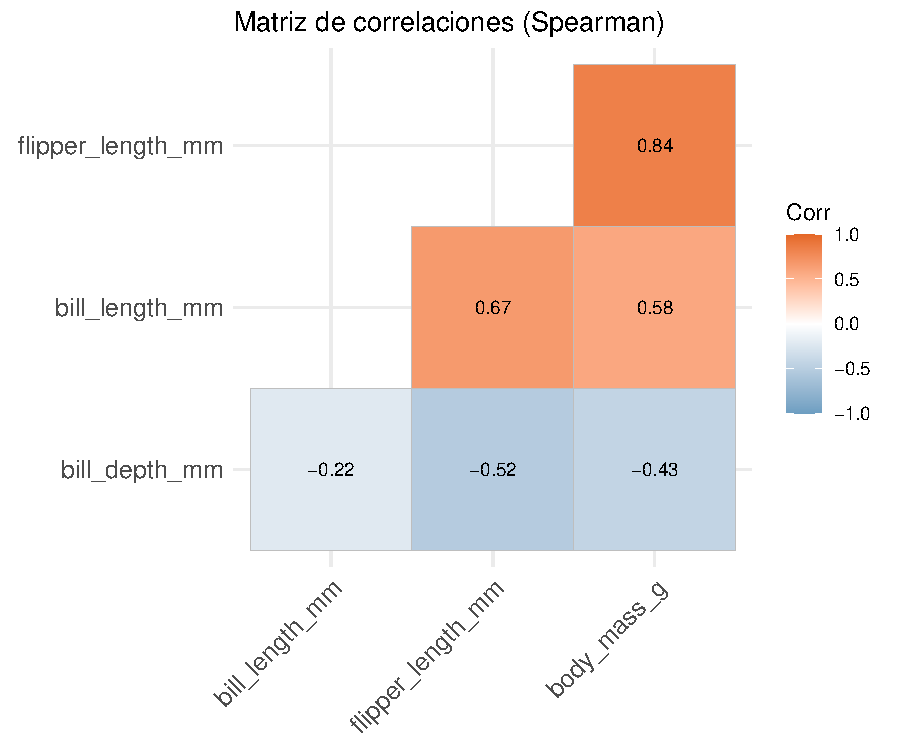
\includegraphics[keepaspectratio]{PCA-nMDS_files/figure-pdf/fig-pca-corr-1.pdf}}

}

\caption{\label{fig-pca-corr}Matriz de correlaciones entre variables
morfométricas (Spearman)}

\end{figure}%

La matriz de correlaciones (Spearman) entre las variables morfométricas
revela patrones claros de asociación entre las dimensiones corporales de
los pingüinos. Las correlaciones más fuertes se observan entre longitud
del aleta y masa corporal (ρ = 0.84), indicando que los individuos con
aletas más largas tienden a ser más pesados. Asimismo, la longitud del
pico se asocia positivamente con ambas variables (ρ ≈ 0.58 a 0.67), lo
que sugiere una coherencia morfológica general: los individuos de mayor
tamaño presentan picos y aletas más desarrollados. Por el contrario, el
ancho del pico muestra correlaciones negativas con las demás medidas (ρ
≈ -0.43 a -0.52), lo que indica que las especies con picos más amchos
tienden a tener aletas más cortas y menor masa corporal (ver
Figura~\ref{fig-pca-corr}).

\section{\texorpdfstring{Ejecutar PCA con \texttt{prcomp()} y extraer
resultados}{Ejecutar PCA con prcomp() y extraer resultados}}\label{ejecutar-pca-con-prcomp-y-extraer-resultados}

\begin{Shaded}
\begin{Highlighting}[numbers=left,,]
\NormalTok{pca\_fit }\OtherTok{\textless{}{-}} \FunctionTok{prcomp}\NormalTok{(df\_pca }\SpecialCharTok{\%\textgreater{}\%} \FunctionTok{select}\NormalTok{(}\FunctionTok{where}\NormalTok{(is.numeric)), }\AttributeTok{scale. =} \ConstantTok{TRUE}\NormalTok{, }
               \AttributeTok{center =} \ConstantTok{TRUE}\NormalTok{)}
\CommentTok{\# Varianza explicada}
\NormalTok{pca\_var }\OtherTok{\textless{}{-}}\NormalTok{ pca\_fit}\SpecialCharTok{$}\NormalTok{sdev}\SpecialCharTok{\^{}}\DecValTok{2}
\NormalTok{pca\_var\_prop }\OtherTok{\textless{}{-}}\NormalTok{ pca\_var }\SpecialCharTok{/} \FunctionTok{sum}\NormalTok{(pca\_var)}

\NormalTok{pca\_summary }\OtherTok{\textless{}{-}} \FunctionTok{tibble}\NormalTok{(}
  \AttributeTok{PC =} \FunctionTok{paste0}\NormalTok{(}\StringTok{"PC"}\NormalTok{, }\FunctionTok{seq\_along}\NormalTok{(pca\_var)),}
  \AttributeTok{sdev =} \FunctionTok{round}\NormalTok{(pca\_fit}\SpecialCharTok{$}\NormalTok{sdev, }\DecValTok{3}\NormalTok{),}
  \AttributeTok{variance =} \FunctionTok{round}\NormalTok{(pca\_var, }\DecValTok{3}\NormalTok{),}
  \AttributeTok{prop.var =} \FunctionTok{round}\NormalTok{(pca\_var\_prop, }\DecValTok{3}\NormalTok{),}
  \AttributeTok{cum.var =} \FunctionTok{round}\NormalTok{(}\FunctionTok{cumsum}\NormalTok{(pca\_var\_prop), }\DecValTok{3}\NormalTok{)}
\NormalTok{)}

\NormalTok{knitr}\SpecialCharTok{::}\FunctionTok{kable}\NormalTok{(pca\_summary)}
\end{Highlighting}
\end{Shaded}

\begin{longtable}[]{@{}lrrrr@{}}

\caption{\label{tbl-pca-fit}Desviaciones, varianza y proporción por
componente}

\tabularnewline

\toprule\noalign{}
PC & sdev & variance & prop.var & cum.var \\
\midrule\noalign{}
\endhead
\bottomrule\noalign{}
\endlastfoot
PC1 & 1.659 & 2.754 & 0.688 & 0.688 \\
PC2 & 0.879 & 0.773 & 0.193 & 0.882 \\
PC3 & 0.604 & 0.365 & 0.091 & 0.973 \\
PC4 & 0.329 & 0.108 & 0.027 & 1.000 \\

\end{longtable}

\section{Gráficos: screeplot y biplot (scores +
loadings)}\label{gruxe1ficos-screeplot-y-biplot-scores-loadings}

\begin{Shaded}
\begin{Highlighting}[numbers=left,,]
\CommentTok{\# Screeplot}
\NormalTok{scree\_df }\OtherTok{\textless{}{-}}\NormalTok{ pca\_summary}
\FunctionTok{ggplot}\NormalTok{(scree\_df, }\FunctionTok{aes}\NormalTok{(}\AttributeTok{x =} \FunctionTok{as.numeric}\NormalTok{(}\FunctionTok{gsub}\NormalTok{(}\StringTok{"PC"}\NormalTok{,}\StringTok{""}\NormalTok{,PC)), }\AttributeTok{y =}\NormalTok{ prop.var)) }\SpecialCharTok{+}
  \FunctionTok{geom\_col}\NormalTok{() }\SpecialCharTok{+}
  \FunctionTok{geom\_line}\NormalTok{(}\FunctionTok{aes}\NormalTok{(}\AttributeTok{y =}\NormalTok{ cum.var), }\AttributeTok{color =} \StringTok{"blue"}\NormalTok{) }\SpecialCharTok{+}
  \FunctionTok{geom\_point}\NormalTok{(}\FunctionTok{aes}\NormalTok{(}\AttributeTok{y =}\NormalTok{ cum.var), }\AttributeTok{color =} \StringTok{"blue"}\NormalTok{) }\SpecialCharTok{+}
  \FunctionTok{labs}\NormalTok{(}\AttributeTok{x =} \StringTok{"Componente principal"}\NormalTok{, }\AttributeTok{y =} \StringTok{"Proporción de varianza explicada"}\NormalTok{,}
       \AttributeTok{title =} \StringTok{"Screeplot PCA"}\NormalTok{) }\SpecialCharTok{+}
  \FunctionTok{theme\_minimal}\NormalTok{()}
\end{Highlighting}
\end{Shaded}

\begin{figure}[H]

\centering{

\pandocbounded{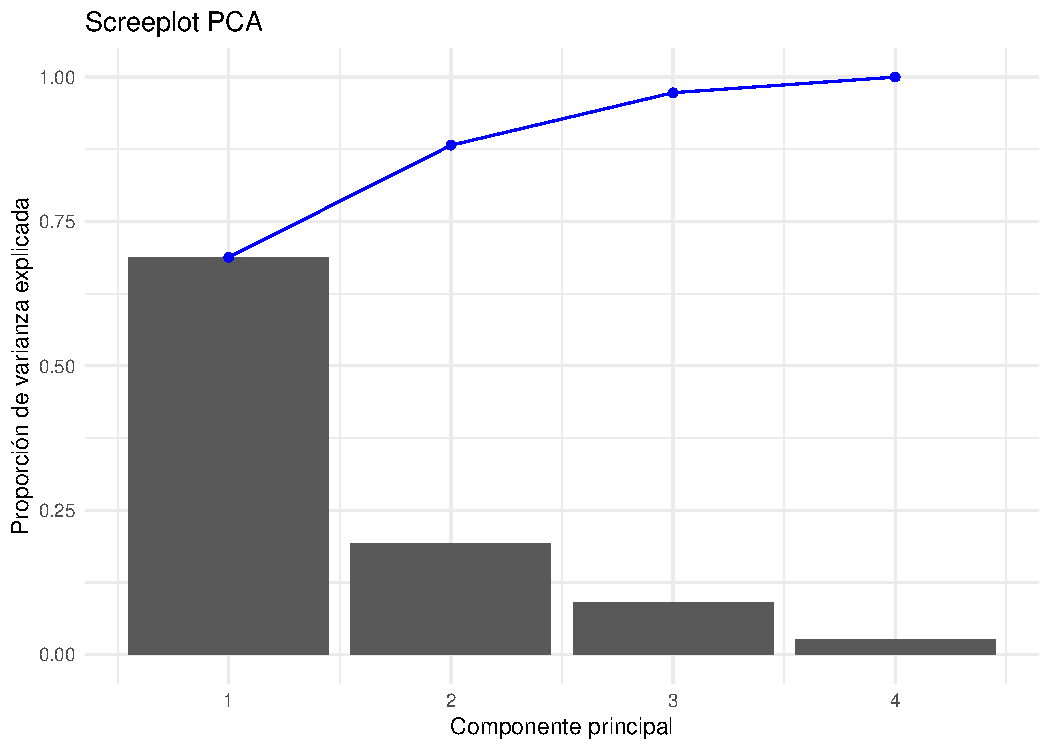
\includegraphics[keepaspectratio]{PCA-nMDS_files/figure-pdf/fig-pca-scree-1.pdf}}

}

\caption{\label{fig-pca-scree}Screeplot PCA:proporción de varianza
explicada por componente}

\end{figure}%

El análisis de componentes principales muestra que las dos primeras
componentes (PC1 y PC2) explican conjuntamente alrededor del 88.2 \% de
la varianza total en las variables morfométricas, lo cual es un nivel de
representación muy adecuado para la reducción de dimensionalidad (ver
Tabla~\ref{tbl-pca-fit} y Figura~\ref{fig-pca-scree}) .

\begin{Shaded}
\begin{Highlighting}[numbers=left,,]
\CommentTok{\# Cargas (loadings) de cada variable en las primeras dos componentes}
\NormalTok{loadings\_tbl }\OtherTok{\textless{}{-}} \FunctionTok{as\_tibble}\NormalTok{(pca\_fit}\SpecialCharTok{$}\NormalTok{rotation[, }\DecValTok{1}\SpecialCharTok{:}\DecValTok{2}\NormalTok{], }\AttributeTok{rownames =} \StringTok{"Variable"}\NormalTok{) }\SpecialCharTok{\%\textgreater{}\%}
  \FunctionTok{rename}\NormalTok{(}\AttributeTok{PC1 =}\NormalTok{ PC1, }\AttributeTok{PC2 =}\NormalTok{ PC2) }\SpecialCharTok{\%\textgreater{}\%}
  \FunctionTok{mutate}\NormalTok{(}\FunctionTok{across}\NormalTok{(}\FunctionTok{where}\NormalTok{(is.numeric), round, }\DecValTok{3}\NormalTok{))}

\NormalTok{knitr}\SpecialCharTok{::}\FunctionTok{kable}\NormalTok{(loadings\_tbl)}
\end{Highlighting}
\end{Shaded}

\begin{longtable}[]{@{}lrr@{}}

\caption{\label{tbl-pca-loadings}Contribución de las variables a los
componentes principales}

\tabularnewline

\toprule\noalign{}
Variable & PC1 & PC2 \\
\midrule\noalign{}
\endhead
\bottomrule\noalign{}
\endlastfoot
bill\_length\_mm & 0.455 & -0.597 \\
bill\_depth\_mm & -0.400 & -0.798 \\
flipper\_length\_mm & 0.576 & -0.002 \\
body\_mass\_g & 0.548 & -0.084 \\

\end{longtable}

La primera componente (PC1), que explica el 68.8 \% de la varianza
total, refleja un gradiente general de tamaño corporal. Las variables
con mayores pesos positivos son \emph{flipper\_length\_mm} (0.576) y
\emph{body\_mass\_g} (0.548), seguidas por \emph{bill\_length\_mm}
(0.455). En contraste, \emph{bill\_depth\_mm} presenta un peso negativo
moderado (-0.400). Esto indica que los individuos con mayores valores en
PC1 tienden a tener alas más largas, mayor masa corporal y picos más
largos pero menos profundos, es decir, una morfología asociada a un
tamaño corporal globalmente mayor (ver Tabla~\ref{tbl-pca-loadings}).

La segunda componente (PC2), que aporta un 19.3 \% adicional de la
varianza, representa principalmente variaciones en la forma del pico.
Aquí destacan los pesos negativos elevados de \emph{bill\_depth\_mm}
(-0.798) y \emph{bill\_length\_mm} (-0.597), lo que sugiere un eje de
contraste entre especies con picos largos y estrechos frente a aquellas
con picos cortos y robustos. Las otras variables
(\emph{flipper\_length\_mm} y \emph{body\_mass\_g}) tienen pesos
cercanos a cero, mostrando poca influencia sobre esta dimensión (ver
Tabla~\ref{tbl-pca-loadings}).

\begin{Shaded}
\begin{Highlighting}[numbers=left,,]
\CommentTok{\# Biplot de variables}
\NormalTok{biplot\_data }\OtherTok{\textless{}{-}} \FunctionTok{as\_tibble}\NormalTok{(pca\_fit}\SpecialCharTok{$}\NormalTok{x[, }\DecValTok{1}\SpecialCharTok{:}\DecValTok{2}\NormalTok{]) }\SpecialCharTok{\%\textgreater{}\%}
  \FunctionTok{mutate}\NormalTok{(}\AttributeTok{species =}\NormalTok{ df\_pca}\SpecialCharTok{$}\NormalTok{species)}

\CommentTok{\# vectores de las variables (loadings)}
\NormalTok{loadings }\OtherTok{\textless{}{-}} \FunctionTok{as.data.frame}\NormalTok{(pca\_fit}\SpecialCharTok{$}\NormalTok{rotation[, }\DecValTok{1}\SpecialCharTok{:}\DecValTok{2}\NormalTok{])}

\FunctionTok{ggplot}\NormalTok{(biplot\_data, }\FunctionTok{aes}\NormalTok{(PC1, PC2, }\AttributeTok{color =}\NormalTok{ species)) }\SpecialCharTok{+}
  \FunctionTok{geom\_point}\NormalTok{(}\AttributeTok{alpha =} \FloatTok{0.7}\NormalTok{, }\AttributeTok{size =} \DecValTok{2}\NormalTok{) }\SpecialCharTok{+}
  \FunctionTok{geom\_segment}\NormalTok{(}\AttributeTok{data =}\NormalTok{ loadings,}
               \FunctionTok{aes}\NormalTok{(}\AttributeTok{x =} \DecValTok{0}\NormalTok{, }\AttributeTok{y =} \DecValTok{0}\NormalTok{, }\AttributeTok{xend =}\NormalTok{ PC1 }\SpecialCharTok{*} \DecValTok{3}\NormalTok{, }\AttributeTok{yend =}\NormalTok{ PC2 }\SpecialCharTok{*} \DecValTok{3}\NormalTok{),}
               \AttributeTok{arrow =} \FunctionTok{arrow}\NormalTok{(}\AttributeTok{length =} \FunctionTok{unit}\NormalTok{(}\FloatTok{0.25}\NormalTok{, }\StringTok{"cm"}\NormalTok{)), }
               \AttributeTok{color =} \StringTok{"black"}\NormalTok{) }\SpecialCharTok{+}
  \FunctionTok{geom\_text\_repel}\NormalTok{(}\AttributeTok{data =}\NormalTok{ loadings,}
                  \FunctionTok{aes}\NormalTok{(}\AttributeTok{x =}\NormalTok{ PC1 }\SpecialCharTok{*} \FloatTok{3.2}\NormalTok{, }\AttributeTok{y =}\NormalTok{ PC2 }\SpecialCharTok{*} \FloatTok{3.2}\NormalTok{, }\AttributeTok{label =} \FunctionTok{rownames}\NormalTok{(loadings)),}
                  \AttributeTok{color =} \StringTok{"black"}\NormalTok{, }\AttributeTok{size =} \FloatTok{3.5}\NormalTok{) }\SpecialCharTok{+}
  \FunctionTok{labs}\NormalTok{(}\AttributeTok{title =} \StringTok{"Biplot PCA: especies y variables morfométricas"}\NormalTok{,}
       \AttributeTok{x =} \StringTok{"Componente 1"}\NormalTok{,}
       \AttributeTok{y =} \StringTok{"Componente 2"}\NormalTok{) }\SpecialCharTok{+}
  \FunctionTok{theme\_minimal}\NormalTok{() }\SpecialCharTok{+}
  \FunctionTok{theme}\NormalTok{(}\AttributeTok{legend.position =} \StringTok{"bottom"}\NormalTok{)}
\end{Highlighting}
\end{Shaded}

\begin{figure}[H]

\centering{

\pandocbounded{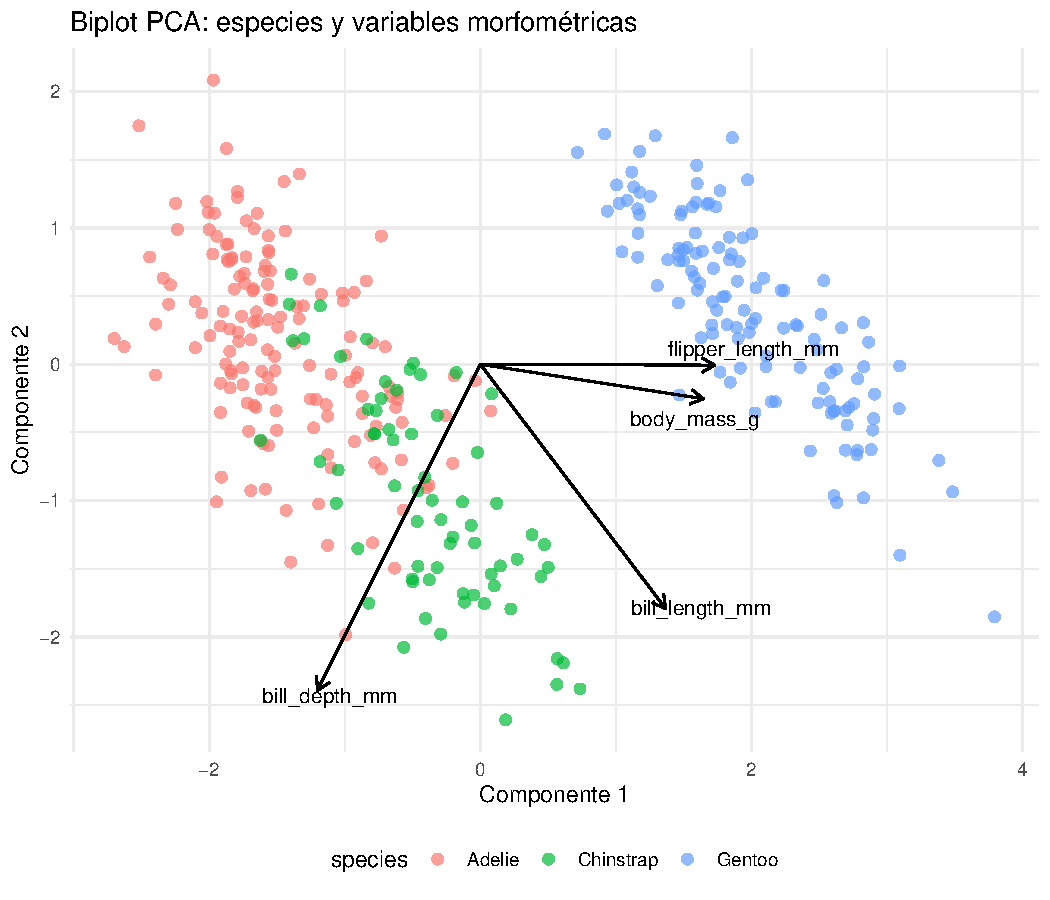
\includegraphics[keepaspectratio]{PCA-nMDS_files/figure-pdf/fig-pca-biplot-1.pdf}}

}

\caption{\label{fig-pca-biplot}Biplot PCA: relación entre variables y
componentes principales}

\end{figure}%

El biplot de componentes principales muestra simultáneamente la posición
de los individuos de cada especie en el espacio definido por los dos
primeros componentes y la dirección de las variables morfométricas que
contribuyen a dicha variación.

El primer componente (PC1) está fuertemente asociado con el tamaño
corporal total, determinado principalmente por las variables
\emph{flipper\_length\_mm} y \emph{body\_mass\_g}, que presentan
vectores largos y orientados en la misma dirección. Las especies con
valores altos en este eje, como \emph{Gentoo}, se agrupan hacia el
extremo positivo del PC1, indicando individuos más grandes y pesados. En
contraste, \emph{Adelie} se concentra en el extremo negativo, reflejando
individuos de menor tamaño (ver Figura~\ref{fig-pca-biplot}).

El segundo componente (PC2) captura variaciones en la morfología del
pico, principalmente asociadas a las variables \emph{bill\_length\_mm} y
\emph{bill\_depth\_mm}. En este eje, \emph{Chinstrap} tiende a ocupar
posiciones intermedias o positivas, caracterizadas por picos más largos
y delgados, mientras que \emph{Adelie} mantiene picos más cortos y
profundos, situándose en la dirección opuesta (ver
Figura~\ref{fig-pca-biplot}).

En síntesis, el análisis de componentes principales permite visualizar
de manera clara la diferenciación morfológica entre las especies de
pingüinos, destacando que el tamaño corporal y la forma del pico son los
principales ejes de variación. Estas diferencias reflejan adaptaciones
específicas de cada especie a su entorno y estrategias alimenticias, lo
que respalda la utilidad del PCA como herramienta para comprender
patrones de variación biológica y relaciones morfométricas entre grupos
cercanos.

\section{Preparación de datos --- transformación Hellinger
(NMDS)}\label{preparaciuxf3n-de-datos-transformaciuxf3n-hellinger-nmds}

\begin{Shaded}
\begin{Highlighting}[numbers=left,,]
\FunctionTok{data}\NormalTok{(varespec)}
\FunctionTok{data}\NormalTok{(varechem)}

\CommentTok{\# Hellinger transforma abundancias para métodos basados en distancia euclidiana,}
\NormalTok{varespec\_hel }\OtherTok{\textless{}{-}} \FunctionTok{decostand}\NormalTok{(varespec, }\AttributeTok{method =} \StringTok{"hellinger"}\NormalTok{)}
\end{Highlighting}
\end{Shaded}

\section{\texorpdfstring{Ejecutar NMDS con \texttt{metaMDS()}
(Bray-Curtis por
defecto)}{Ejecutar NMDS con metaMDS() (Bray-Curtis por defecto)}}\label{ejecutar-nmds-con-metamds-bray-curtis-por-defecto}

\begin{Shaded}
\begin{Highlighting}[numbers=left,,]
\CommentTok{\# Ajuste del NMDS (sin mostrar mensajes de ejecución)}
\FunctionTok{set.seed}\NormalTok{(}\DecValTok{42}\NormalTok{)}
\FunctionTok{suppressMessages}\NormalTok{(\{}
  \FunctionTok{capture.output}\NormalTok{(\{}
\NormalTok{    nmds }\OtherTok{\textless{}{-}} \FunctionTok{metaMDS}\NormalTok{(}
\NormalTok{      varespec\_hel,}
      \AttributeTok{distance =} \StringTok{"bray"}\NormalTok{,}
      \AttributeTok{k =} \DecValTok{2}\NormalTok{,}
      \AttributeTok{trymax =} \DecValTok{100}\NormalTok{,}
      \AttributeTok{autotransform =} \ConstantTok{FALSE}
\NormalTok{    )}
\NormalTok{  \})}
\NormalTok{\})}
\end{Highlighting}
\end{Shaded}

\begin{Shaded}
\begin{Highlighting}[numbers=left,,]
\CommentTok{\# Curva de ajuste (stressplot)}
\NormalTok{vegan}\SpecialCharTok{::}\FunctionTok{stressplot}\NormalTok{(nmds)}
\end{Highlighting}
\end{Shaded}

\begin{figure}[H]

\centering{

\pandocbounded{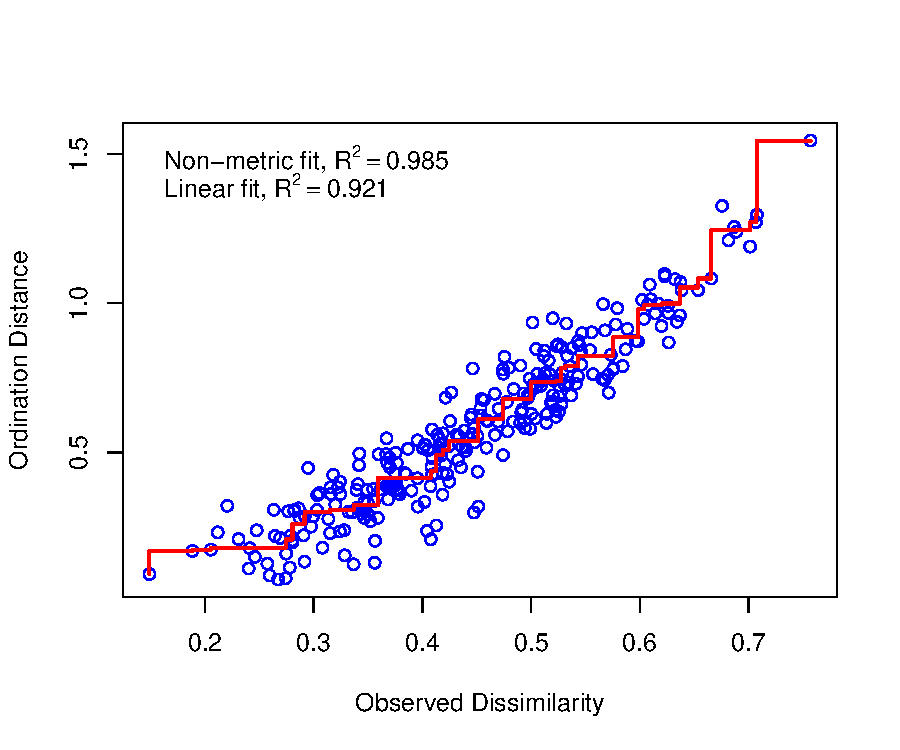
\includegraphics[keepaspectratio]{PCA-nMDS_files/figure-pdf/fig-nmds-stress-1.pdf}}

}

\caption{\label{fig-nmds-stress}Curva de ajuste NMDS (stressplot) para
evaluar la calidad del ordenamiento}

\end{figure}%

El análisis de escala multidimensional no métrica (NMDS) alcanzó un
valor de \emph{stress} de 0.12, lo cual indica una representación
bidimensional adecuada según los criterios de Kruskal (valores
\textless{} 0.2 son aceptables, y \textless{} 0.1 excelentes). Los
indicadores de ajuste complementarios refuerzan la calidad del
ordenamiento: Non-metric fit R² = 0.985: sugiere que el 98.5 \% de la
variación en las distancias rankeadas se preserva en el espacio de dos
dimensiones. Linear fit R² = 0.921: indica una alta correspondencia
lineal entre las distancias originales y las del NMDS (ver
Figura~\ref{fig-nmds-stress}).

\section{Visualización NMDS: sitios + especies +
envfit}\label{visualizaciuxf3n-nmds-sitios-especies-envfit}

\begin{Shaded}
\begin{Highlighting}[numbers=left,,]
\CommentTok{\# Ajustar variables ambientales (envfit)}
\NormalTok{ef }\OtherTok{\textless{}{-}} \FunctionTok{envfit}\NormalTok{(nmds, varechem, }\AttributeTok{permutations =} \DecValTok{999}\NormalTok{)}

\CommentTok{\# Extraer resultados del envfit}
\NormalTok{ef\_results }\OtherTok{\textless{}{-}} \FunctionTok{as.data.frame}\NormalTok{(ef}\SpecialCharTok{$}\NormalTok{vectors}\SpecialCharTok{$}\NormalTok{arrows)}
\NormalTok{ef\_r2 }\OtherTok{\textless{}{-}}\NormalTok{ ef}\SpecialCharTok{$}\NormalTok{vectors}\SpecialCharTok{$}\NormalTok{r}
\NormalTok{ef\_p }\OtherTok{\textless{}{-}}\NormalTok{ ef}\SpecialCharTok{$}\NormalTok{vectors}\SpecialCharTok{$}\NormalTok{pvals}

\CommentTok{\# Crear tabla resumen}
\NormalTok{tabla\_envfit }\OtherTok{\textless{}{-}}\NormalTok{ ef\_results }\SpecialCharTok{\%\textgreater{}\%}
  \FunctionTok{rownames\_to\_column}\NormalTok{(}\StringTok{"Variable"}\NormalTok{) }\SpecialCharTok{\%\textgreater{}\%}
  \FunctionTok{mutate}\NormalTok{(}
    \AttributeTok{R2 =} \FunctionTok{round}\NormalTok{(ef\_r2, }\DecValTok{3}\NormalTok{),}
    \AttributeTok{p\_value =} \FunctionTok{signif}\NormalTok{(ef\_p, }\DecValTok{3}\NormalTok{),}
    \AttributeTok{NMDS1 =} \FunctionTok{round}\NormalTok{(NMDS1, }\DecValTok{3}\NormalTok{),}
    \AttributeTok{NMDS2 =} \FunctionTok{round}\NormalTok{(NMDS2, }\DecValTok{3}\NormalTok{)}
\NormalTok{  ) }\SpecialCharTok{\%\textgreater{}\%}
  \FunctionTok{arrange}\NormalTok{(}\FunctionTok{desc}\NormalTok{(R2))}

\NormalTok{knitr}\SpecialCharTok{::}\FunctionTok{kable}\NormalTok{(}
\NormalTok{  tabla\_envfit,}
  \AttributeTok{align =} \StringTok{"lcccc"}
\NormalTok{)}
\end{Highlighting}
\end{Shaded}

\begin{longtable}[]{@{}lcccc@{}}

\caption{\label{tbl-nmds-envfit}Resultados del ajuste de variables
ambientales (envfit) sobre el espacio NMDS}

\tabularnewline

\toprule\noalign{}
Variable & NMDS1 & NMDS2 & R2 & p\_value \\
\midrule\noalign{}
\endhead
\bottomrule\noalign{}
\endlastfoot
Mn & 0.999 & 0.043 & 0.468 & 0.001 \\
Humdepth & 0.994 & 0.110 & 0.466 & 0.003 \\
Al & -0.981 & 0.196 & 0.460 & 0.002 \\
Fe & -0.970 & 0.244 & 0.414 & 0.003 \\
Ca & 0.959 & 0.284 & 0.308 & 0.020 \\
Mg & 0.998 & 0.065 & 0.223 & 0.077 \\
P & 0.882 & 0.471 & 0.217 & 0.084 \\
pH & -0.875 & 0.484 & 0.215 & 0.069 \\
K & 0.954 & 0.300 & 0.195 & 0.104 \\
Baresoil & 0.889 & -0.458 & 0.184 & 0.123 \\
Zn & 0.954 & -0.300 & 0.149 & 0.178 \\
N & -0.024 & -1.000 & 0.091 & 0.339 \\
Mo & -0.606 & -0.796 & 0.076 & 0.429 \\
S & 0.853 & 0.522 & 0.040 & 0.658 \\

\end{longtable}

Los resultados del ajuste de variables ambientales sobre el espacio de
ordenamiento NMDS (ver Tabla~\ref{tbl-nmds-envfit}) permiten cuantificar
la influencia de cada factor edáfico sobre la composición de especies.
Los valores de R² indican la fuerza de la relación entre cada variable y
la estructura de la comunidad, mientras que los valores de p reflejan su
significancia estadística.

Las variables Mn, Humdepth, Al y Fe muestran los valores de R² más altos
(≥ 0.41, \emph{p} \textless{} 0.01), lo que evidencia que son los
principales controladores de la variación observada. Mn y Humdepth se
orientan hacia el cuadrante derecho del diagrama, representando sitios
con suelos más fértiles, mayor contenido de materia orgánica y
disponibilidad de nutrientes. En contraste, Al y Fe apuntan hacia el
cuadrante izquierdo, definiendo un gradiente de acidez y metalización,
asociado a suelos menos fértiles y más restrictivos para el crecimiento
vegetal.

Un segundo grupo de variables, con valores intermedios de R² (entre 0.20
y 0.30), incluye Ca, Mg, P y pH. Estas variables refuerzan el eje
principal del ordenamiento: mientras Ca, Mg y P se agrupan hacia la
derecha, representando la fertilidad edáfica, el pH (con sentido
opuesto) marca el extremo ácido de dicho gradiente.

Finalmente, variables como K, Baresoil, Zn, N, Mo y S presentan valores
bajos de R² (\textless{} 0.20) y sin significancia estadística (\emph{p}
\textgreater{} 0.05), por lo que su contribución a la organización
global de las comunidades es menor. No obstante, podrían reflejar
variaciones locales o efectos secundarios asociados a la exposición,
perturbación o heterogeneidad microambiental.

En conjunto, los resultados del \emph{envfit} confirman que el
ordenamiento NMDS está estructurado principalmente por un gradiente de
fertilidad--acidez del suelo, donde la composición vegetal responde a la
disponibilidad de nutrientes y a las condiciones edáficas que limitan o
favorecen el desarrollo de las especies.

\begin{Shaded}
\begin{Highlighting}[numbers=left,,]
\CommentTok{\# Extraer coordenadas de sitios}
\NormalTok{sites\_scores }\OtherTok{\textless{}{-}} \FunctionTok{as\_tibble}\NormalTok{(}\FunctionTok{scores}\NormalTok{(nmds, }\AttributeTok{display =} \StringTok{"sites"}\NormalTok{)) }\SpecialCharTok{\%\textgreater{}\%}
  \FunctionTok{mutate}\NormalTok{(}\AttributeTok{site =} \FunctionTok{rownames}\NormalTok{(varespec))}

\CommentTok{\# Extraer coordenadas de especies}
\NormalTok{species\_scores }\OtherTok{\textless{}{-}} \FunctionTok{as\_tibble}\NormalTok{(}\FunctionTok{scores}\NormalTok{(nmds, }\AttributeTok{display =} \StringTok{"species"}\NormalTok{)) }\SpecialCharTok{\%\textgreater{}\%}
  \FunctionTok{rownames\_to\_column}\NormalTok{(}\StringTok{"species"}\NormalTok{)}

\CommentTok{\# Ajustar variables ambientales (envfit)}
\NormalTok{ef }\OtherTok{\textless{}{-}} \FunctionTok{envfit}\NormalTok{(nmds, varechem, }\AttributeTok{permutations =} \DecValTok{999}\NormalTok{)}

\CommentTok{\# Mantener nombres correctos de variables ambientales}
\NormalTok{ef\_arrows }\OtherTok{\textless{}{-}} \FunctionTok{as.data.frame}\NormalTok{(ef}\SpecialCharTok{$}\NormalTok{vectors}\SpecialCharTok{$}\NormalTok{arrows)}
\NormalTok{ef\_arrows}\SpecialCharTok{$}\NormalTok{var }\OtherTok{\textless{}{-}} \FunctionTok{rownames}\NormalTok{(ef\_arrows)}
\NormalTok{ef\_arrows }\OtherTok{\textless{}{-}}\NormalTok{ ef\_arrows }\SpecialCharTok{\%\textgreater{}\%}
  \FunctionTok{as\_tibble}\NormalTok{() }\SpecialCharTok{\%\textgreater{}\%}
  \FunctionTok{rename}\NormalTok{(}\AttributeTok{NMDS1 =}\NormalTok{ NMDS1, }\AttributeTok{NMDS2 =}\NormalTok{ NMDS2)}

\CommentTok{\# Gráfico NMDS con vectores ambientales}
\FunctionTok{ggplot}\NormalTok{(sites\_scores, }\FunctionTok{aes}\NormalTok{(}\AttributeTok{x =}\NormalTok{ NMDS1, }\AttributeTok{y =}\NormalTok{ NMDS2)) }\SpecialCharTok{+}
  \FunctionTok{geom\_point}\NormalTok{(}\AttributeTok{size =} \DecValTok{3}\NormalTok{, }\AttributeTok{alpha =} \FloatTok{0.8}\NormalTok{) }\SpecialCharTok{+}
  \FunctionTok{geom\_text\_repel}\NormalTok{(}\FunctionTok{aes}\NormalTok{(}\AttributeTok{label =}\NormalTok{ site), }\AttributeTok{size =} \DecValTok{3}\NormalTok{, }\AttributeTok{max.overlaps =} \DecValTok{15}\NormalTok{) }\SpecialCharTok{+}
  \FunctionTok{geom\_segment}\NormalTok{(}
    \AttributeTok{data =}\NormalTok{ ef\_arrows,}
    \FunctionTok{aes}\NormalTok{(}\AttributeTok{x =} \DecValTok{0}\NormalTok{, }\AttributeTok{y =} \DecValTok{0}\NormalTok{, }\AttributeTok{xend =}\NormalTok{ NMDS1, }\AttributeTok{yend =}\NormalTok{ NMDS2),}
    \AttributeTok{arrow =} \FunctionTok{arrow}\NormalTok{(}\AttributeTok{length =} \FunctionTok{unit}\NormalTok{(}\FloatTok{0.25}\NormalTok{, }\StringTok{"cm"}\NormalTok{)),}
    \AttributeTok{color =} \StringTok{"black"}
\NormalTok{  ) }\SpecialCharTok{+}
  \FunctionTok{geom\_text\_repel}\NormalTok{(}
    \AttributeTok{data =}\NormalTok{ ef\_arrows,}
    \FunctionTok{aes}\NormalTok{(}\AttributeTok{x =}\NormalTok{ NMDS1, }\AttributeTok{y =}\NormalTok{ NMDS2, }\AttributeTok{label =}\NormalTok{ var),}
    \AttributeTok{size =} \DecValTok{3}\NormalTok{,}
    \AttributeTok{color =} \StringTok{"black"}
\NormalTok{  ) }\SpecialCharTok{+}
  \FunctionTok{labs}\NormalTok{(}
    \AttributeTok{title =} \FunctionTok{paste0}\NormalTok{(}\StringTok{"NMDS (stress = "}\NormalTok{, }\FunctionTok{round}\NormalTok{(nmds}\SpecialCharTok{$}\NormalTok{stress, }\DecValTok{3}\NormalTok{), }\StringTok{")"}\NormalTok{),}
    \AttributeTok{x =} \StringTok{"NMDS1"}\NormalTok{,}
    \AttributeTok{y =} \StringTok{"NMDS2"}
\NormalTok{  ) }\SpecialCharTok{+}
  \FunctionTok{theme\_minimal}\NormalTok{()}
\end{Highlighting}
\end{Shaded}

\begin{figure}[H]

\centering{

\pandocbounded{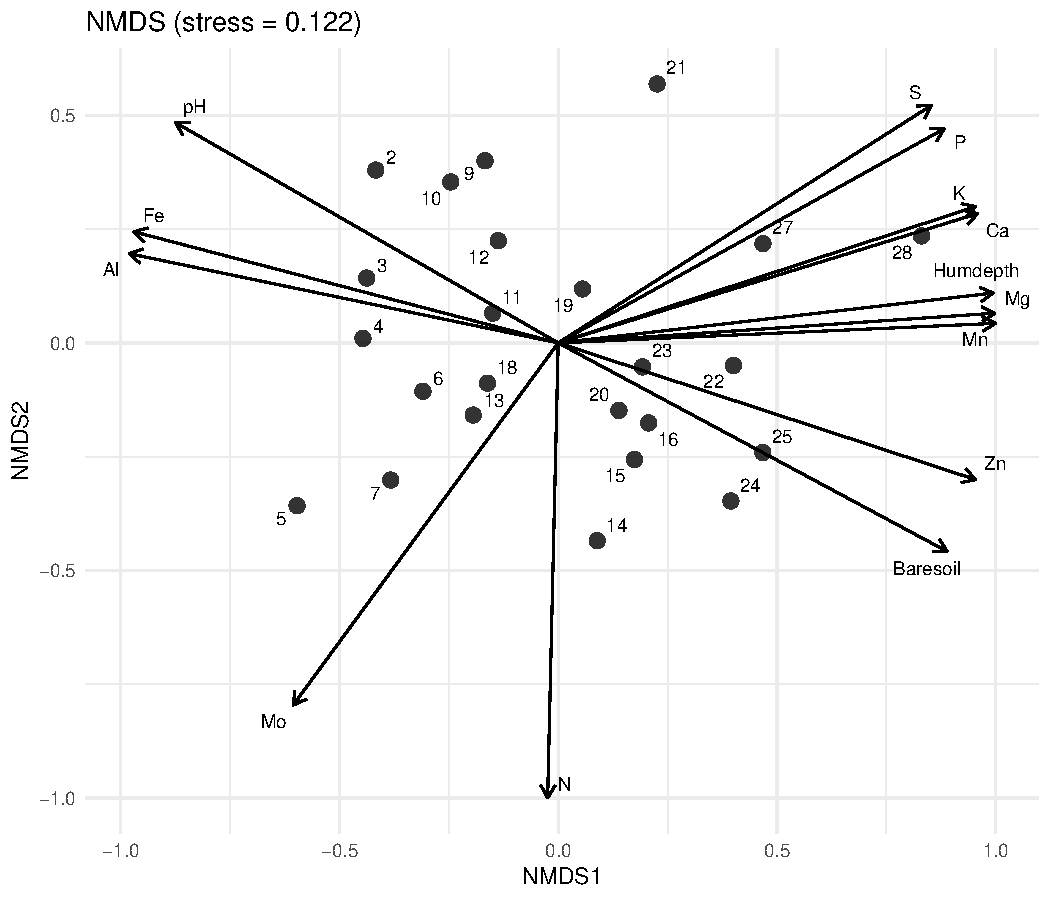
\includegraphics[keepaspectratio]{PCA-nMDS_files/figure-pdf/fig-nmds-biplot-1.pdf}}

}

\caption{\label{fig-nmds-biplot}Ordenamiento NMDS basado en distancias
de Bray--Curtis, con ajuste de variables ambientales mediante envfit}

\end{figure}%

El biplot del NMDS representa la estructura de similitud entre los
sitios en función de la composición de especies (varespec), incorporando
además los gradientes ambientales medidos en cada sitio (varechem). Los
vectores ambientales indican la dirección y magnitud de las variables
que mejor explican la variación en la comunidad biológica: cuanto más
largos y definidos, mayor es su poder explicativo sobre la distribución
de las especies (ver Figura~\ref{fig-nmds-biplot}).

El nitrógeno (N) muestra un vector orientado hacia la parte inferior del
eje NMDS2, lo que sugiere que los sitios en esa dirección presentan
concentraciones elevadas de este nutriente y comunidades asociadas a
ambientes más enriquecidos.

Las variables S (azufre), P (fósforo), K (potasio) y Ca (calcio) apuntan
hacia el cuadrante superior derecho del diagrama, indicando que los
sitios en esta región se asocian a suelos más fértiles y con mayor
disponibilidad de nutrientes, donde predominan especies adaptadas a
condiciones más productivas.

Por otro lado, pH, Fe (hierro) y Al (aluminio) se orientan hacia el
cuadrante superior izquierdo, definiendo un gradiente de acidez y
metalización. Los sitios en esta dirección tienden a presentar suelos
más ácidos y menos fértiles, lo que puede restringir el crecimiento
vegetal y favorecer especies tolerantes a condiciones edáficas
limitantes.

Las variables Baresoil (suelo desnudo) y Zn (zinc) apuntan hacia el
cuadrante inferior derecho, lo que podría reflejar sitios más abiertos o
degradados, con menor cobertura vegetal y condiciones más extremas o
expuestas.

Además, la proximidad entre los vectores de S, P, K y Ca indica que
estas variables co-varían positivamente, definiendo un eje de fertilidad
edáfica. En cambio, la orientación opuesta de pH, Fe y Al revela un
gradiente inverso de acidez y metalización, contrapuesto a la
fertilidad. Por su parte, el nitrógeno (N) mantiene una posición
relativamente independiente, lo que sugiere que su variación no está
directamente alineada con los principales gradientes ambientales.

La posición de los sitios en el espacio NMDS refuerza estas
asociaciones:

\begin{itemize}
\item
  Los sitios cercanos entre sí (por ejemplo, 1, 3, 9, 10 y 12) presentan
  una composición florística similar, vinculada con suelos ácidos y
  altos contenidos de Fe y Al.
\item
  En contraste, los sitios 14, 15, 24 y 25 se agrupan hacia el extremo
  inferior derecho, asociados a altos valores de Zn y mayor proporción
  de suelo desnudo, característicos de hábitats más empobrecidos o
  erosionados.
\item
  Algunos sitios más dispersos, como 21 o 27, podrían representar zonas
  de transición ecológica, donde confluyen gradientes intermedios de
  fertilidad y acidez.
\end{itemize}

En conjunto, el ordenamiento NMDS muestra una estructura clara donde los
patrones de composición de especies se explican principalmente por
gradientes edáficos de fertilidad, acidez y contenido metálico,
evidenciando la fuerte influencia del ambiente físico sobre la
organización ecológica de las comunidades.

\section{Conclusiones}\label{conclusiones}

El análisis de componentes principales permitió reducir cuatro variables
morfométricas a dos ejes biológicamente interpretables, PC1 (68.8 \%):
gradiente de tamaño corporal general.y PC2 (19.3 \%): gradiente de forma
del pico. Estos resultados confirman que las diferencias entre
\emph{Adelie}, \emph{Chinstrap} y \emph{Gentoo} responden principalmente
a contrastes en masa corporal, longitud de aleta y morfología del pico,
variables estrechamente vinculadas con la ecología trófica y las
estrategias adaptativas de cada especie.

En síntesis, el NMDS evidenció que la estructura de las comunidades
vegetales está fuertemente condicionada por gradientes de fertilidad
(definido por concentraciones de S, P, K y Ca) y acidez del suelo
(explicado por pH, Fe y Al), y constituye un método flexible y poderoso
para explorar patrones ecológicos complejos, incluso en escenarios con
datos no normales o altamente heterogéneos.




\end{document}
